
	\section{Computación Paralela}

	La computación paralela es el uso de múltiples recursos computacionales para resolver un problema o una necesidad de computo en particular. La computación paralela surge como respuesta ante la necesidad de incrementar los recursos, sea en procesador, memoria y así mejorar el tiempo de respuesta para problemas con alta complejidad computacional o alto volumen de análisis de datos. 

	El paradigma computacional tradicional ha sido de computación serial, donde una tarea es dividida en una serie finita de instrucciones que son ejecutada de forma secuencial, donde una sola instrucción es ejecutada en un momento dado. 

	La computación paralela rompe el paradigma anterior, buscando que en un momento dado se puedan ejecutar varias instrucciones, utilizando múltiples procesadores y una entidad que orqueste los mismos.\cite{LLNL} \cite{SC}

	\section{Apolo}

	%\todo[inline,caption={TODO}]{Arquitectura de apolo. Redes.}

	\section{Grafos}

	Los grafos son abstracciones matemáticas que son útiles a la hora de resolver muchos tipos de problemas en las ciencias de la computación. Un grafo es un conjunto ordenado de nodos y vertices. 

	Nodos

	Vertices

	donde los vértices son relaciones entre los nodos. 

	La aplicación de la teoría de grafos permite un estudio de relaciones entre sus nodos. 



	\begin{figure}[H]
		\centering
		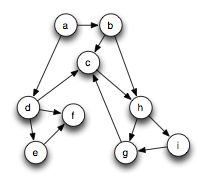
\includegraphics[width=0.25\textwidth]{aux/grafo}
		\caption[Estructura de un Grafo]{
		(tomada de \cite{BoostGrafos})}
		%\label{F-dimensions-emotion}
	\end{figure}


	\begin{figure}[H]
		\centering
		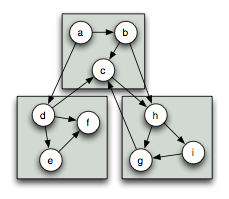
\includegraphics[width=0.25\textwidth]{aux/distributed-graph}
		\caption[Grafo Distribuido]{
		(tomada de \cite{BoostGrafos})}
		%\label{F-dimensions-emotion}
	\end{figure}
	

	\begin{figure}[H]
		\centering
		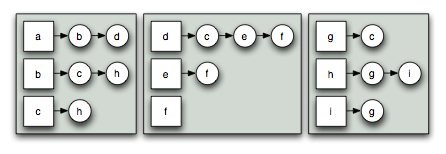
\includegraphics[width=0.5\textwidth]{aux/dist-adjlist}
		\caption[Grafo en lista de adyacencia]{
		(tomada de \cite{BoostGrafos})}
		%\label{F-dimensions-emotion}
	\end{figure}


	\begin{figure}[H]
		\centering
		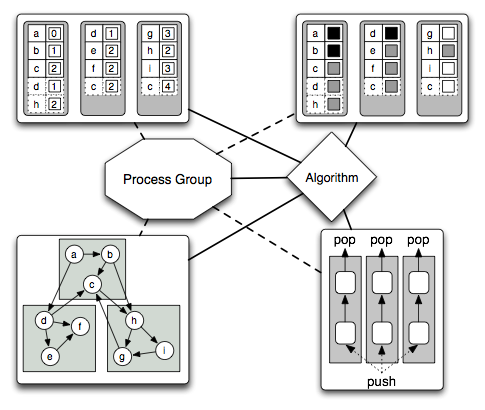
\includegraphics[width=0.5\textwidth]{aux/arquitectura_grafos}
		\caption[Aquitectura de Grafos]{
		(tomada de \cite{BoostGrafos})}
		%\label{F-dimensions-emotion}
	\end{figure}
	

	\section{C++}

	C++ es un lenguaje de programación de propositos generales,  que soporta abstracción de datos, es multiparadigma (programación estructurada, programación generica\cite{andrei2001modern} y programación orientada a objetos).

	C++ fue la elegido para este proyecto por su buen uso de los recursos computacionales, ampliamente reconocido como un lenguaje altamente eficiente, muy veloz y potente. \cite{stroustrup2013c++}


	\section{MPI}

	MPI es un sistema de paso de mensajes diseñado para permitir la comunicación entre varias unidades de computo, este surgio como un mecanismo para resolver la necesidad de permitir que multiples procesos en paralelo trabajen de manera concurrente hacia la solución de un problema en particular.   \cite{Karniadakis}

	\section{Boost}

	Boost son una serie de librerias de C++, implementadas y mejoradas por la comunidad cuya base es el buen funcionamiento con la Libreria Estandar de C++ (C++ STL) y la eventual estandarización de las mismas, mediante el mejoramiento progresivo de estas.\cite{wwwBoost}

	Boost dentro de sus librerias tiene implementaciónes de programación generica para grafos y adicionalmente una libreria de algoritmos paralelos para grafos. 


	\section{Parallel Boost Graph Library}

	La PBGL es una librería de Boost para Grafos de Boost para computación paralela y distribuida. Esta ofrece algoritmos para computación en paralelo y distribuida, conservando las mismas interfaces que la librería secuencia para grafos de Boost.\cite{wwwBoost} 
